

Monaural speech enhancement aims to estimate a clean speech signal from a single-channel mixture corrupted by noise. Deploying enhancement algorithms in real-time applications like live communication or smart home assistants presents a significant challenge, as it demands not only high-quality output but also fast processing speed on resource-limited devices.

Early traditional approaches like spectral subtraction or Wiener filtering \cite{spectral-subtraction} focused on estimating spectral amplitude of clean speech. However, they rely on noise stationarity assumption and often fail in real-world environments. Other techniques exploited the periodicity of voiced speech \cite{adaptive-comb, adaptive-filt}, but they require accurate pitch information. Furthermore, while many of these traditional techniques improve speech quality, they often fail to enhance speech intelligibility \cite{lim-oppenheim-1979}.
%The advent of deep neural networks (DNNs) has marked a paradigm shift in speech enhancement. By learning complex, nonlinear mappings from noisy to clean speech in a data-driven manner,
In contrast, deep neural network (DNN)-based models have demonstrated a remarkable ability to handle diverse noise types, significantly surpassing traditional methods \cite{deep-se-overview}. Nonetheless, the high computational demands of these models result in significant processing latency on resource-constrained devices, hindering their deployment on real-world products.
%In response, there has been growing interest in designing efficient real-time streaming speech enhancement networks.

\begin{figure}[htp]
    \centerline{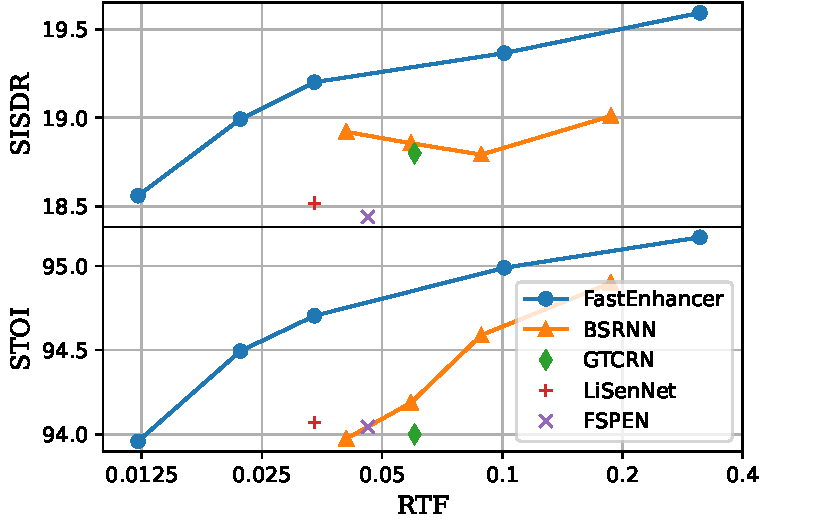
\includegraphics[width=1.0\linewidth]{fig_main.pdf}}
    \vspace{-0.4cm}
    \caption{RTF vs. SISDR and RTF vs. STOI of various models.}
    \label{fig:main}
\end{figure}

In response, many recent studies have attempted to decrease the number of parameters or multiply-accumulate (MAC) operations of neural speech enhancement models. These attempts include dual-path recurrent neurat network (DPRNN) structures \cite{dprnn, dpcrn, trunet}, elaborate encoder–decoder designs \cite{gtcrn}, and sub-band decomposition strategies \cite{fspen, lisennet, bsrnn-se, bsrnn-music-separation}. Although these approaches successfully reduce the number of parameters and MAC operations, we observe that they frequently increase memory operations and architectural complexity, which slows down the actual inference speed (Section \ref{sec:related-speed}). Furthermore, despite the widespread adoption of DPRNN, it remains an open question whether it is the optimal structure, particularly concerning its assumption of a sequential relationship between frequency bands (Section \ref{sec:related-dpn}).

% Many recent models have focused on reducing computational load by introducing complicated and elaborate encoder-decoder and dual path recurrent neural network (DPRNN) structures \cite{dprnn, dpcrn, trunet, gtcrn}. Others have decomposed input spectrograms into multiple sub-bands, processing them with separate networks to better capture local information \cite{fspen, lisennet, bsrnn-se, bsrnn-music-separation}. Although these strategies reduce the number of parameters or multiply-accumulate (MAC) operations, we observe that they frequently increase memory operations and architectural complexity, which slows down the actual inference speed on resource-constrained devices (Section \ref{sec:related-speed}). Furthermore, despite the widespread adoption of DPRNN, it remains an open question whether it is the optimal structure, particularly concerning its assumption of a sequential relationship between frequency bands (Section \ref{sec:related-dpn}).

To address these limitations, we focus on developing a neural speech enhancement model that satisfies the following properties:
\begin{itemize}[itemsep=0pt,leftmargin=1em]
    \item \textbf{High quality and intelligibility}: The enhanced speech sounds clear and natural (high quality), with the words being easy to understand (high intelligibility).
    \item \textbf{Streaming}: The model can process input spectrograms in a frame-by-frame manner.
    \item \textbf{Fast processing speed}: The model achieves a low real-time factor (RTF) on resource-constrained environments, where RTF is the ratio of processing time to the input audio duration. We consider a single CPU thread as a key benchmark for such environments, as many real-world applications lack dedicated hardware accelerators like GPUs or NPUs.
\end{itemize}

To meet these objectives, we introduce \textit{FastEnhancers}, a family of streaming neural speech enhancement models optimized for speed, quality, and intelligibility. Our key contributions are:
\begin{itemize}[itemsep=0pt,leftmargin=1em]
    \item We demonstrate that a streamlined encoder-decoder structure, in contrast to the complex, sub-band-focused designs of prior works, improves processing speed without sacrificing performance.
    \item We propose an RNNFormer block, an efficient dual-path block that combines a time-axis recurrent neural network (RNN) for low-complexity temporal modeling with a frequency-axis transformer for effectively capturing global, non-sequential relationships across frequency bands.
    \item We evaluate \textit{FastEnhancers} against existing models using various metrics for speech quality and intelligibility on the VCTK-Demand dataset \cite{vctk-demand}. Experimental results show that \textit{FastEnhancers} achieve state-of-the-art performances and the lowest RTFs among all evaluated models. By configuring models with various speeds, we establish a new Pareto frontier for the trade-off between the model performance and inference speed (Fig. \ref{fig:main}).
\end{itemize}

